\documentclass[border=4pt]{standalone}
\usepackage{tikz}
\usetikzlibrary{arrows.meta,calc}

\begin{document}
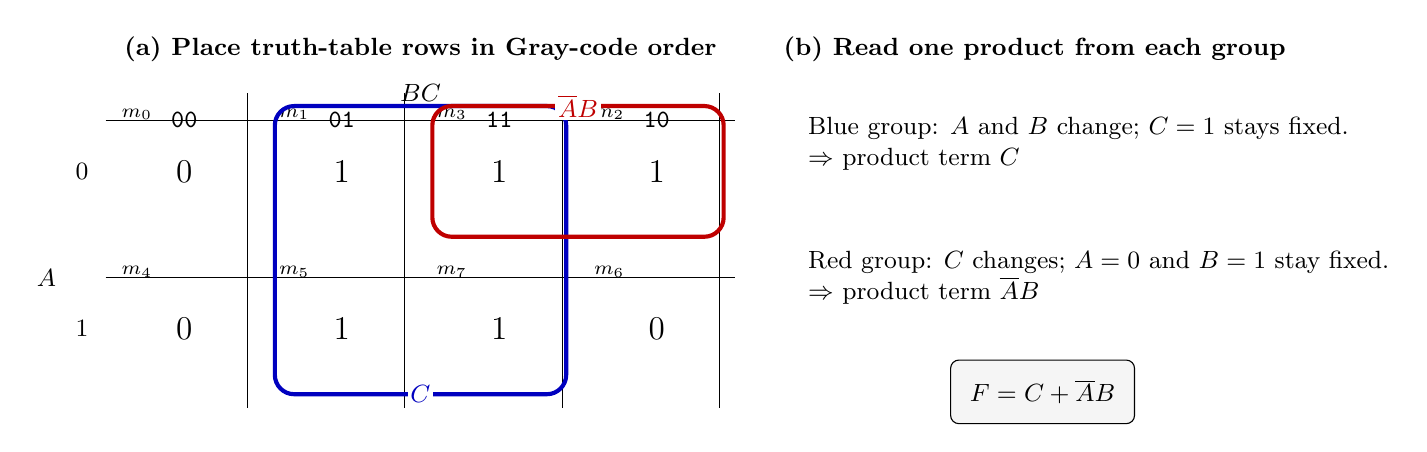
\begin{tikzpicture}[font=\small, >=Latex]
  \node[font=\small\bfseries] at (4.2,4.9)
    {(a) Place truth-table rows in Gray-code order};
  \node at (-0.55,2.0) {$A$};
  \node at (4.2,4.35) {$BC$};
  \node at (-0.1,3.35) {$0$};
  \node at (-0.1,1.35) {$1$};
  \foreach \x/\lab in {0/00,1/01,2/11,3/10}
    \node at ({1.2+2*\x},4.0) {\texttt{\lab}};
  \draw (0.2,0.35) grid[xstep=2,ystep=2] (8.2,4.35);
  \foreach \x/\y/\m/\v in {
    0/0/0/0,1/0/1/1,2/0/3/1,3/0/2/1,
    0/1/4/0,1/1/5/1,2/1/7/1,3/1/6/0}
  {
    \node[font=\scriptsize, anchor=north west] at ({0.28+2*\x},{4.27-2*\y}) {$m_{\m}$};
    \node[font=\large] at ({1.2+2*\x},{3.35-2*\y}) {\v};
  }
  \draw[blue!75!black, line width=1.5pt, rounded corners=7pt]
    (2.35,0.52) rectangle (6.05,4.18);
  \node[blue!75!black, fill=white, inner sep=1pt] at (4.2,0.52) {$C$};
  \draw[red!75!black, line width=1.5pt, rounded corners=7pt]
    (4.35,2.52) rectangle (8.05,4.18);
  \node[red!75!black, fill=white, inner sep=1pt] at (6.2,4.18)
    {$\overline A B$};

  \node[font=\small\bfseries] at (12.0,4.9)
    {(b) Read one product from each group};
  \node[align=left, anchor=west] at (9.0,3.7)
    {Blue group: $A$ and $B$ change; $C=1$ stays fixed.\\
     $\Rightarrow$ product term $C$};
  \node[align=left, anchor=west] at (9.0,2.0)
    {Red group: $C$ changes; $A=0$ and $B=1$ stay fixed.\\
     $\Rightarrow$ product term $\overline A B$};
  \node[draw, rounded corners=3pt, fill=gray!8, inner sep=7pt]
    at (12.1,0.55) {$F=C+\overline A B$};
\end{tikzpicture}
\end{document}
